\documentclass[a4paper, 10pt, final, garamond]{book}
\usepackage{cours-preambule}
\graphicspath{{./figures/}}

\makeatletter
\renewcommand{\@chapapp}{Contr\^ole de connaissances}
\makeatother

% \toggletrue{student}
% \HideSolutionstrue

\begin{document}
\setcounter{chapter}{3}

\chapter{Électrocinétique~: condensateurs et bobines}

\ifstudent{
	\begin{tikzpicture}[remember picture, overlay]
		\node[anchor=north west, align=left]
		at ([shift={(1.4cm,0)}]current page.north west)
		{\\[5pt]\Large\bfseries Nom~:\\[10pt]\Large\bfseries Prénom~:};
		\node[anchor=north east, align=right]
		at ([shift={(-1.5cm,-17pt)}]current page.north east)
		{\Large\bfseries Note~:\hspace{1cm}/10};
	\end{tikzpicture}
}

\begin{enumerate}[label=\sqenumi, leftmargin=10pt]
	\nitem{5}
	\noindent
	\begin{minipage}[t]{.69\linewidth}
		On suppose le circuit RC série suivant, en échelon de tension montant. On
		suppose le condensateur initialement déchargé, et on ferme l'interupteur à
		$t=0$. Déterminer l'équation différentielle sous forme canonique de $u_C$
		pour $t \geq 0$, donner la condition initiale et comment la déterminer, et
		résoudre l'équation différentielle.
	\end{minipage}
	\hfill
	\begin{minipage}[t]{.29\linewidth}
		~
		\vspace{-30pt}
		\begin{center}
			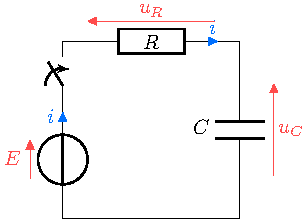
\includegraphics[width=.7\linewidth]{circ_rc-start}
			\captionof{figure}{}
		\end{center}
	\end{minipage}
	\begin{isd}[sidebyside align=top]
		\wsw{
		Avec la loi des mailles,
		\begin{DispWithArrows*}
			u_R + u_C &= E
			\Arrow{$u_R = Ri$\\et $i = C \dv{u_C}{t}$}
			\\\Lra
			RC \dv{u_C}{t} + u_C        & = E
			\Arrow{$\tau = RC$}
			\\\Lra
			\dv{u_C}{t} + \frac{1}{\tau}u_C & = \frac{E}{\tau}
		\end{DispWithArrows*}
		L'équation homogène est~:
		\[
			\dv{u_{C,h}}{t} + \frac{1}{\tau}u_{C,h} = 0
		\]
		La forme générale de la solution pour cette équation est~:
		\[
			u_{C,h}(t) = A\exp\left( -\frac{t}{\tau} \right)
		\]
		}
		\tcblower
		\wsw{
			Une solution particulière avec $u_{C,p}(t) = \lambda$ donne
			\[
				0 + \frac{\lambda}{\tau} = \frac{E}{\tau}
			\]
			Donc $u_{C,p}(t) = E$ est \textbf{une} solution de l'équation
			différentielle.
			La solution générale est donc
			\[
				u_C(t) = E + A\exp \left( - \frac{t}{\tau} \right)
			\]
			La condition initiale est, par continuité de $u_C(t)$,
			\[
				u_C(t=0) = 0
				\qqet
				u_C(0) = A + E \Ra A=-E
			\]
			Ainsi,
			\[
				\boxed{u_C(t) = E\left(1-\exp\left(-\frac{t}{\tau}\right)\right)}
			\]
		}
	\end{isd}
	\nitem{5} Démontrer, à l'aide d'un schéma, l'association série de deux
	condensateurs, ainsi que l'association parallèle de deux bobines.
	\smallbreak
	\begin{isd}
		\begin{center}
			\switch{
				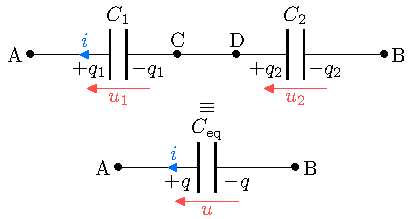
\includegraphics[width=.7\linewidth, draft=true]{cserie}
			}{
				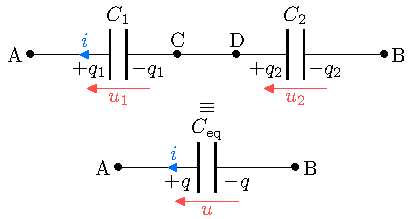
\includegraphics[width=.7\linewidth]{cserie}
			}
			\captionof{figure}{C en série}
		\end{center}
		\wsw{
			Les deux points C et D sont au même potentiel. On déduit ainsi
			\begin{gather*}
				u_{CD} = u_{C} - u_{D} = 0 \Lra q_2 - q_1 = 0
				\\\Lra
				\boxed{q_2 = q_1 = q}
			\end{gather*}
			Ainsi,
			\begin{DispWithArrows*}
				u & = u_1 + u_2
				\Arrow{$q=Cu$}
				\\\Lra
				u & = \frac{q}{C_1} + \frac{q}{C_2}
				\\\Lra
				u & = \left(\frac{1}{C_1} + \frac{1}{C_2}\right)q
			\end{DispWithArrows*}
			On a bien l'expression d'un unique condensateur de capacité
			\fbox{$\frac{1}{C_{\rm eq}} = \frac{1}{C_1} + \frac{1}{C_2}$}
		}
		\vspace{-15pt}
		\tcblower
		\begin{center}
			\switch{
				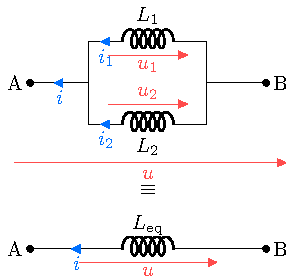
\includegraphics[width=.5\linewidth, draft=true]{bpara}
			}{
				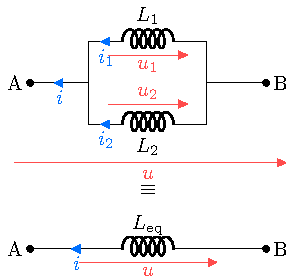
\includegraphics[width=.5\linewidth]{bpara}
			}
			\captionof{figure}{L en parallèle}
		\end{center}
		\wsw{
			\begin{DispWithArrows*}[]
				i &= i_1+i_2
				\Arrow{$\dv{t}(~)$}
				\\\Ra
				\dv{i}{t} &= \dv{i_1}{t} + \dv{i_2}{t}
				\Arrow{$u_L = L \dv{i}{t}$}
				\\\Lra
				\frac{u}{L_{\rm eq}} &= \frac{u}{L_1} + \frac{u}{L_2}
			\end{DispWithArrows*}
			On a bien l'expression d'une unique bobine d'inductance
			\[
				\boxed{\dfrac{1}{L_{\rm eq}} = \dfrac{1}{L_1} + \dfrac{1}{L_2}}
			\]
		}
	\end{isd}
\end{enumerate}
\vspace{-15pt}
\end{document}
